\section{Risultati numerici}
\begin{frame}
\tableofcontents[currentsection]
\end{frame}

\begin{frame}
\frametitle{Convergenza DRDR}

{\footnotesize
\begin{equation}
\begin{split}
& C_1(x,y)=\frac{70}{1+x}(-\frac{2}{3L_y} y^3+ y^2) \psp{7}
C_2(x,z)=\frac{70}{1+x}(-\frac{2}{3L_z}z^3+z^2) \\
& u_{es}(x,y,z)=10^5exp( - \frac{\chi}{\mu L_y} (y - Ly/2 )^2 + C_1  - \frac{\chi}{\mu L_z}(z - L_z/2 ) ^ 2 + C_2 )(Lx-x)^2 
\end{split}
\end{equation}
}\\

\begin{figure}[!h]
\centering
{\linkimage{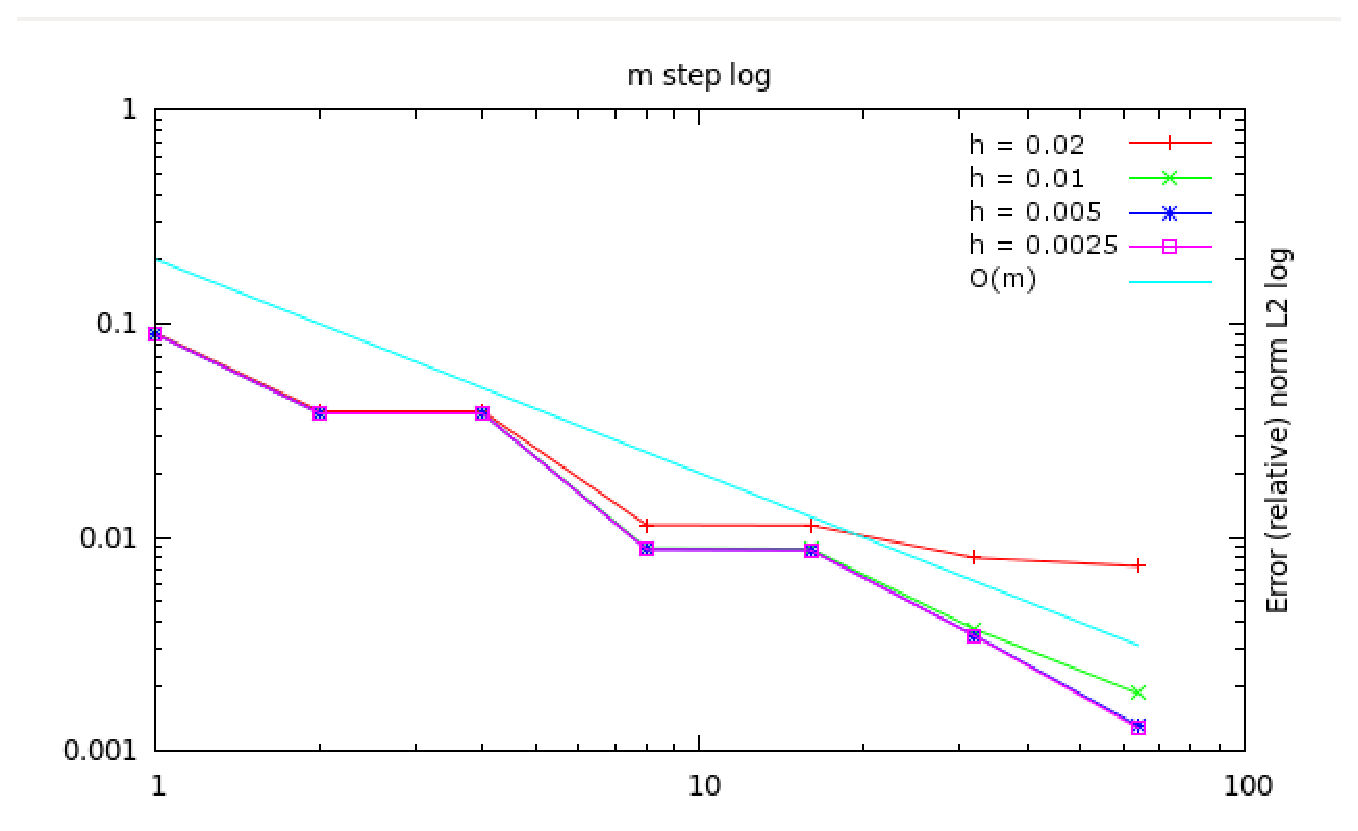
\includegraphics[scale=0.32]{Convergenze/DRDR}}{Convergenze/DRDR}}
\label{fig:drdrconv}
\end{figure}
\end{frame}

\begin{frame}
\frametitle{Convergenza RRRR}
{\footnotesize
\begin{equation}
\begin{split}
& C_1(x,y)=\frac{70}{1+x}(-\frac{2}{3L_y} y^3+ y^2) \psp{7}
C_2(x,z)=\frac{70}{1+x}(-\frac{2}{3L_z}z^3+z^2) \\
& u_{es}(x,y,z)=10^5exp( - \frac{\chi}{\mu L_y} (y - Ly/2 )^2 + C_1  - \frac{\chi}{\mu L_z}(z - L_z/2 ) ^ 2 + C_2 )(Lx-x)^2 
\end{split}
\end{equation}
}
\begin{figure}[!h]
\centering
{\linkimage{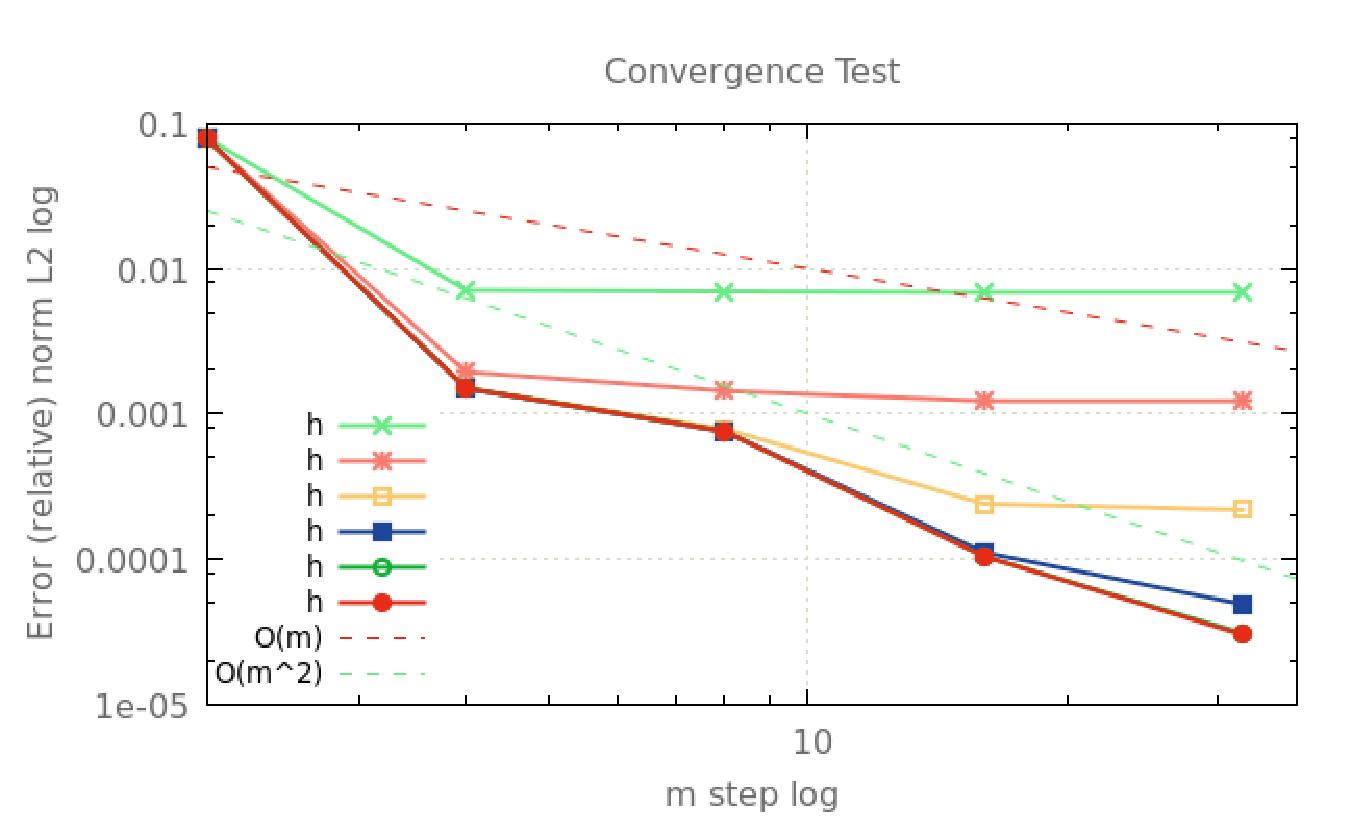
\includegraphics[scale=0.32]{Convergenze/RRRR}}{Convergenze/RRRR}}
\end{figure}

\end{frame}

\begin{frame}
\frametitle{Test camini}
\begin{columns}
\begin{column}{0.5 \paperwidth}
\begin{equation}
\label{eq: problema forte}
\begin{cases}
-\mu\Delta u + \vect{b}\cdot \nabla u + \sigma u = f & \text{in $\Omega$}\\
u=u_{in} & \text{su $\Gamma_{in}$}\\
\frac{\partial u}{\partial \vect{n}}=0 & \text{su $\Gamma_{out}$ }\\
u=0 & \text{su $\Gamma _{vaso}$} \\
\end{cases}
\end{equation}
\begin{figure}
{\linkimage{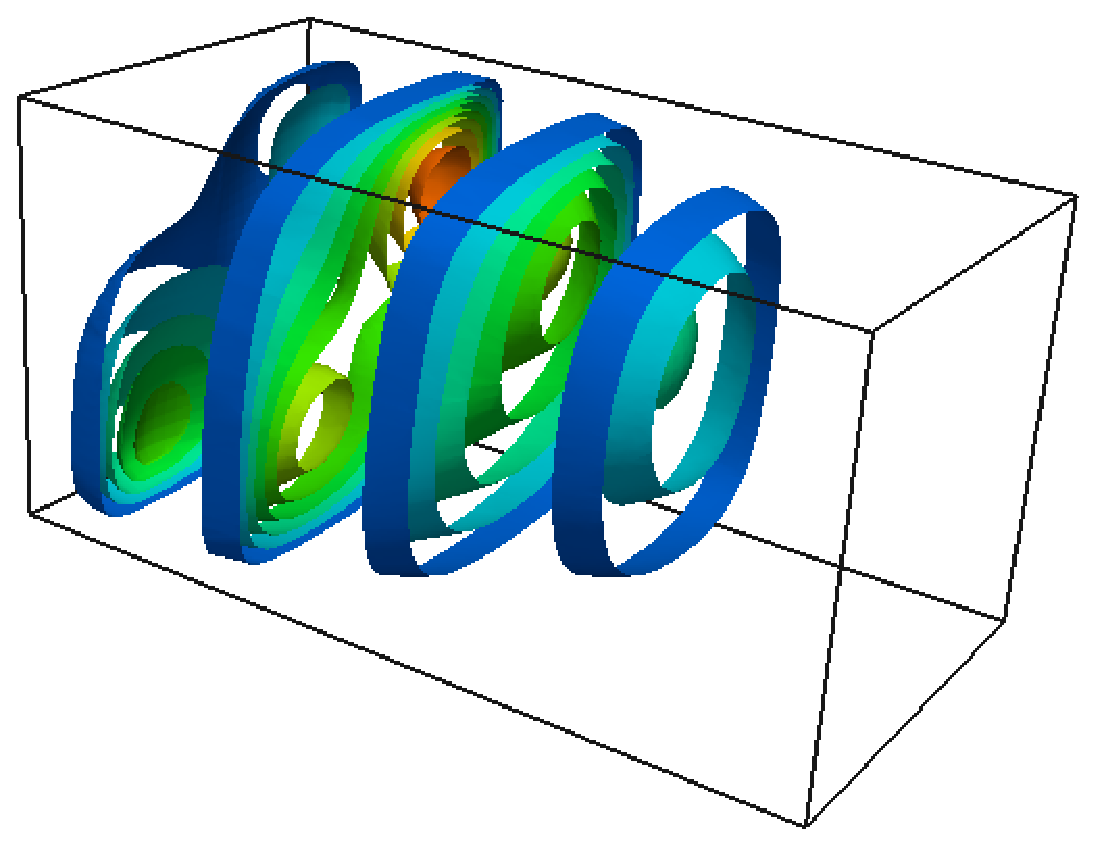
\includegraphics[scale=0.3]{Foto2D+/HiModPretty50}}{Foto2D+/HiModPretty50}}
\end{figure}
\end{column}

\begin{column}{0.5 \paperwidth}
\begin{figure}
\subfigure
{\linkimage{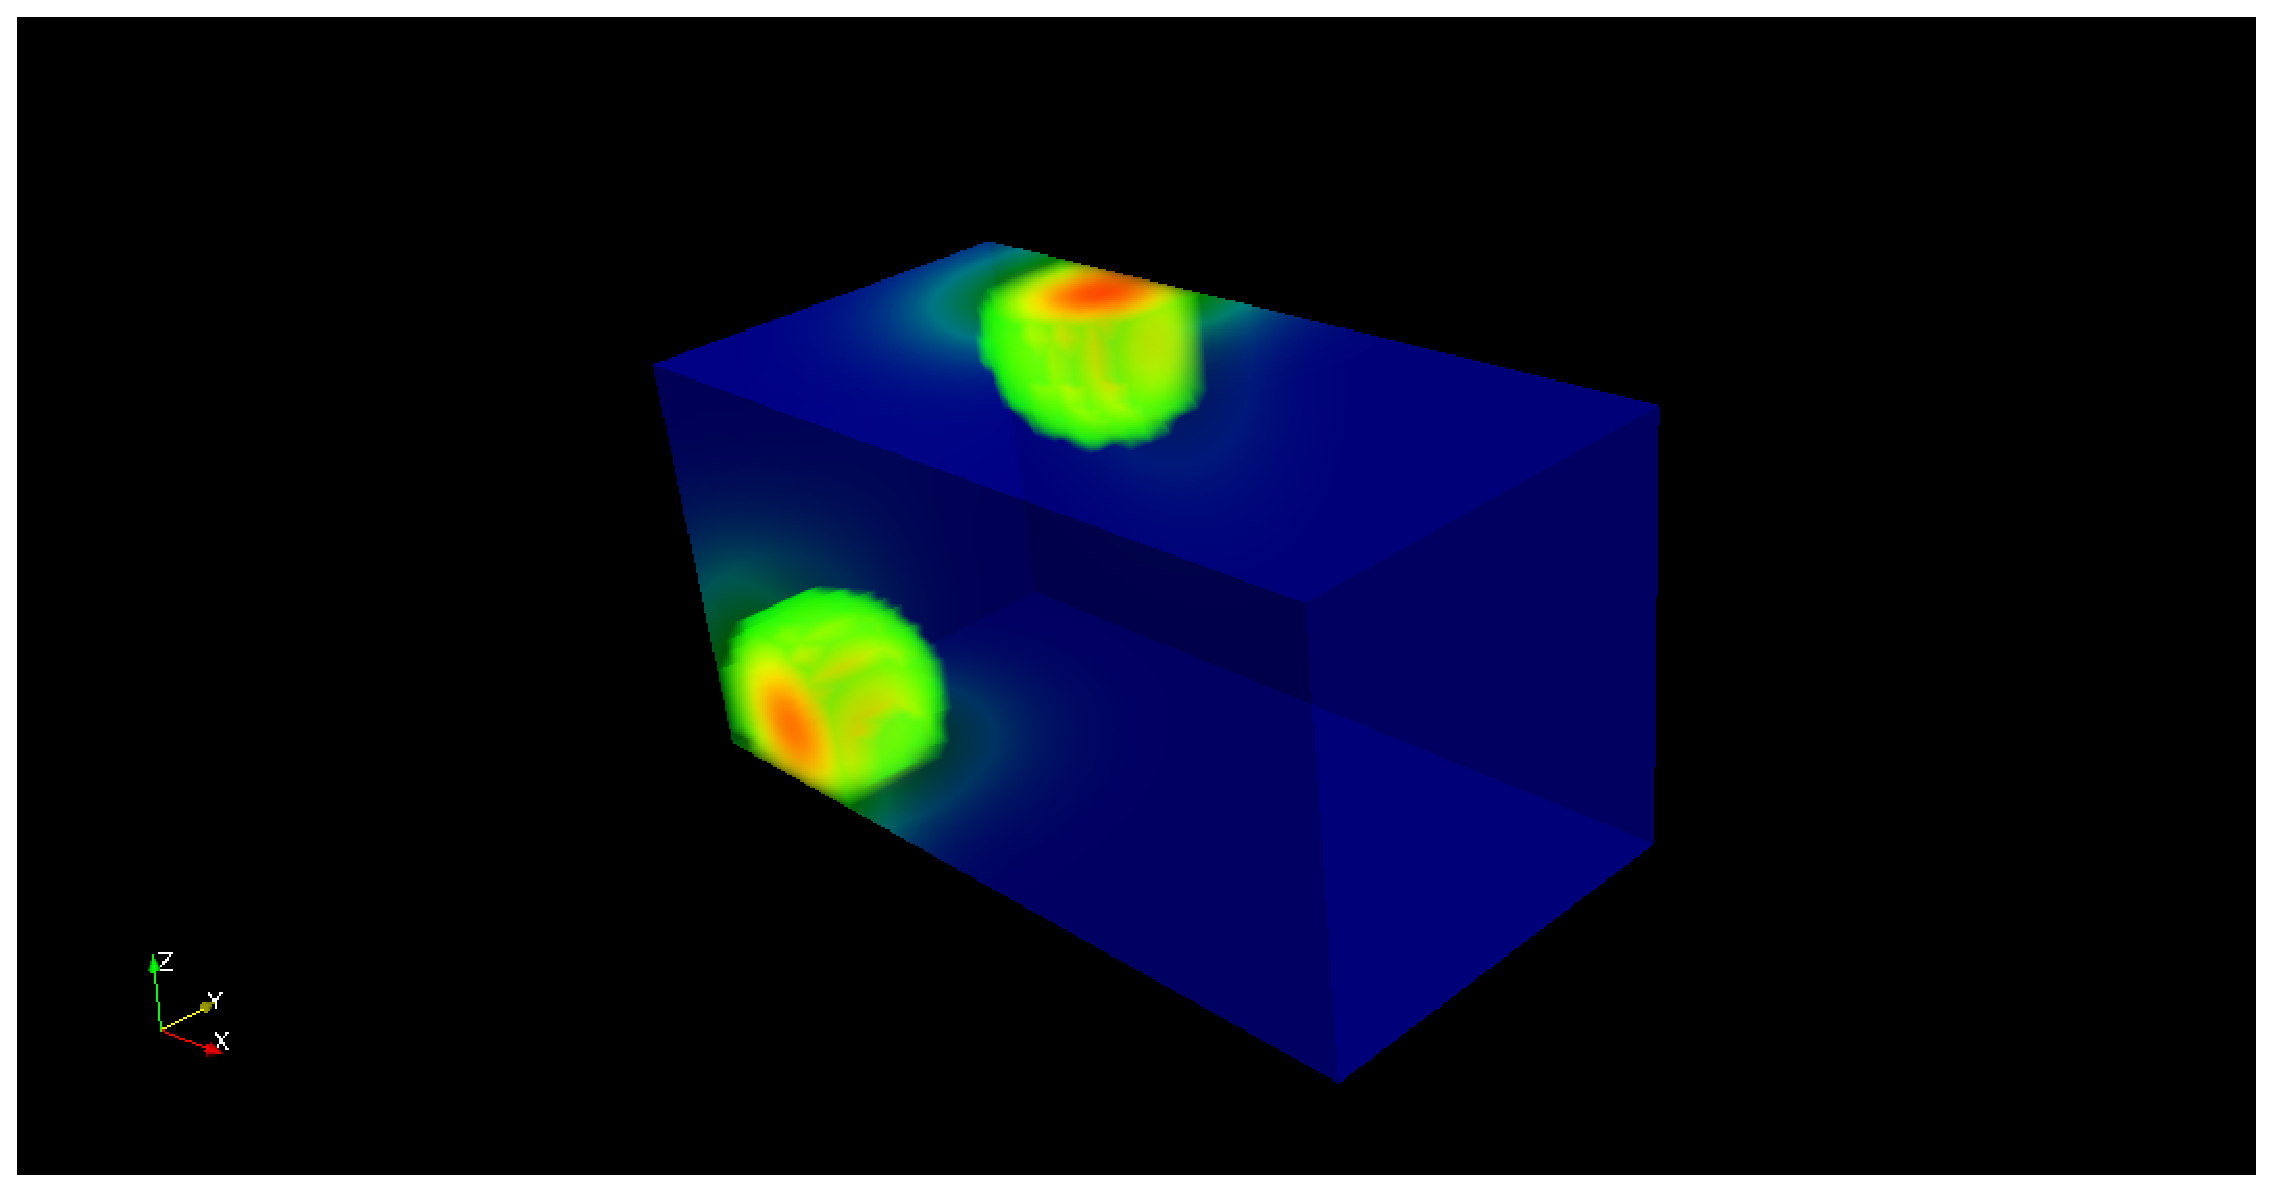
\includegraphics[scale=0.22]{DDDD_ADR/Forceterm}}{DDDD_ADR/Forceterm}}
\subfigure
{\linkimage{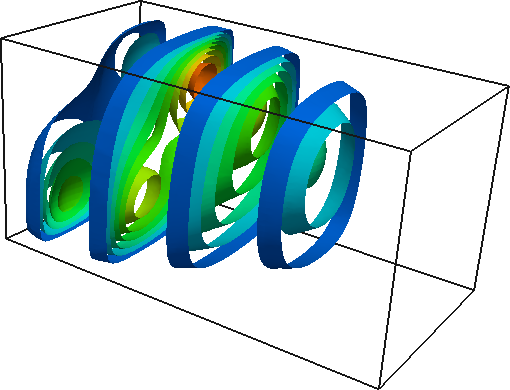
\includegraphics[scale=0.3]{Foto2D+/FEMPretty}}{Foto2D+/FEMPretty}}
\end{figure}
\end{column}

\end{columns}
\end{frame}

\begin{frame}
\frametitle{Slice XY 2D}

\begin{columns}

\begin{column}{0.5 \paperwidth}
\begin{figure}
\subfigure[m=9]
{\linkimage{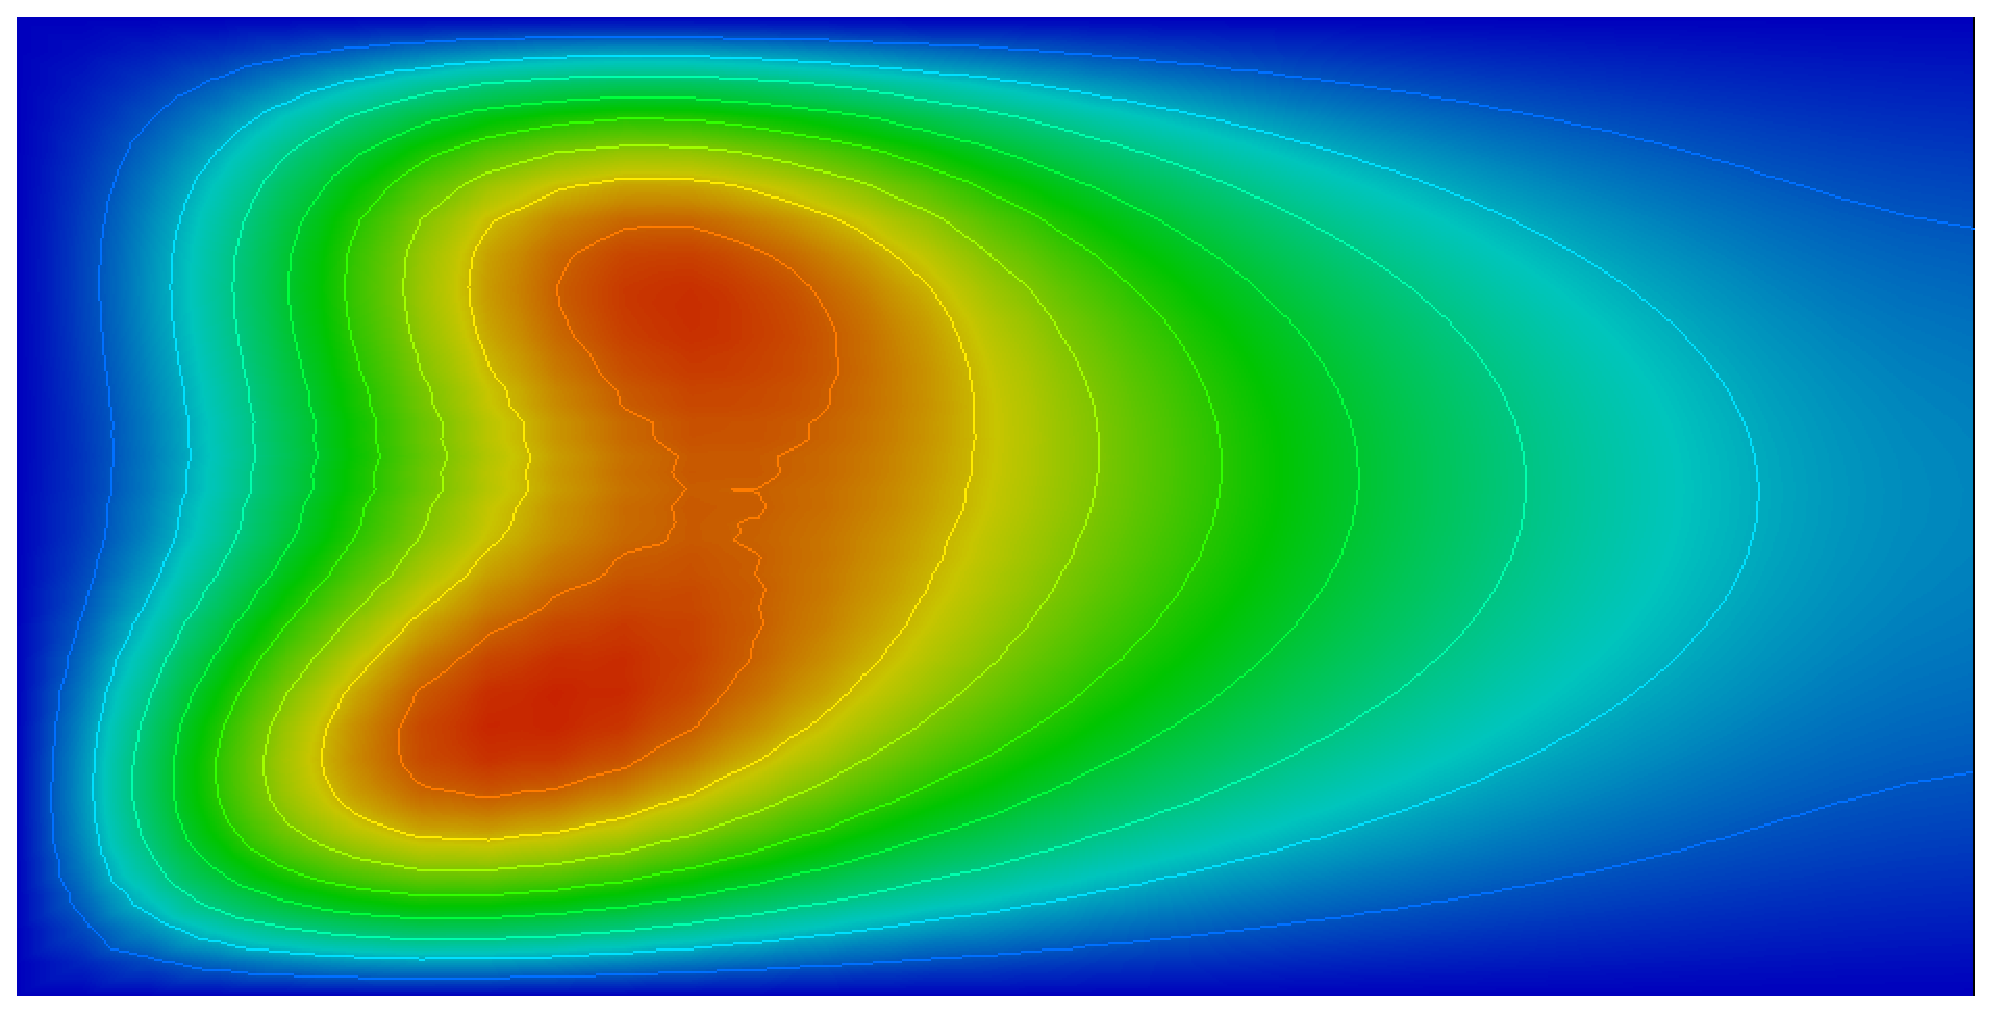
\includegraphics[height=2.8cm,width=5.5cm]{DDDD_ADR/HiMod9slice}}{DDDD_ADR/HiMod9slice}}
\subfigure[m=25]
{\linkimage{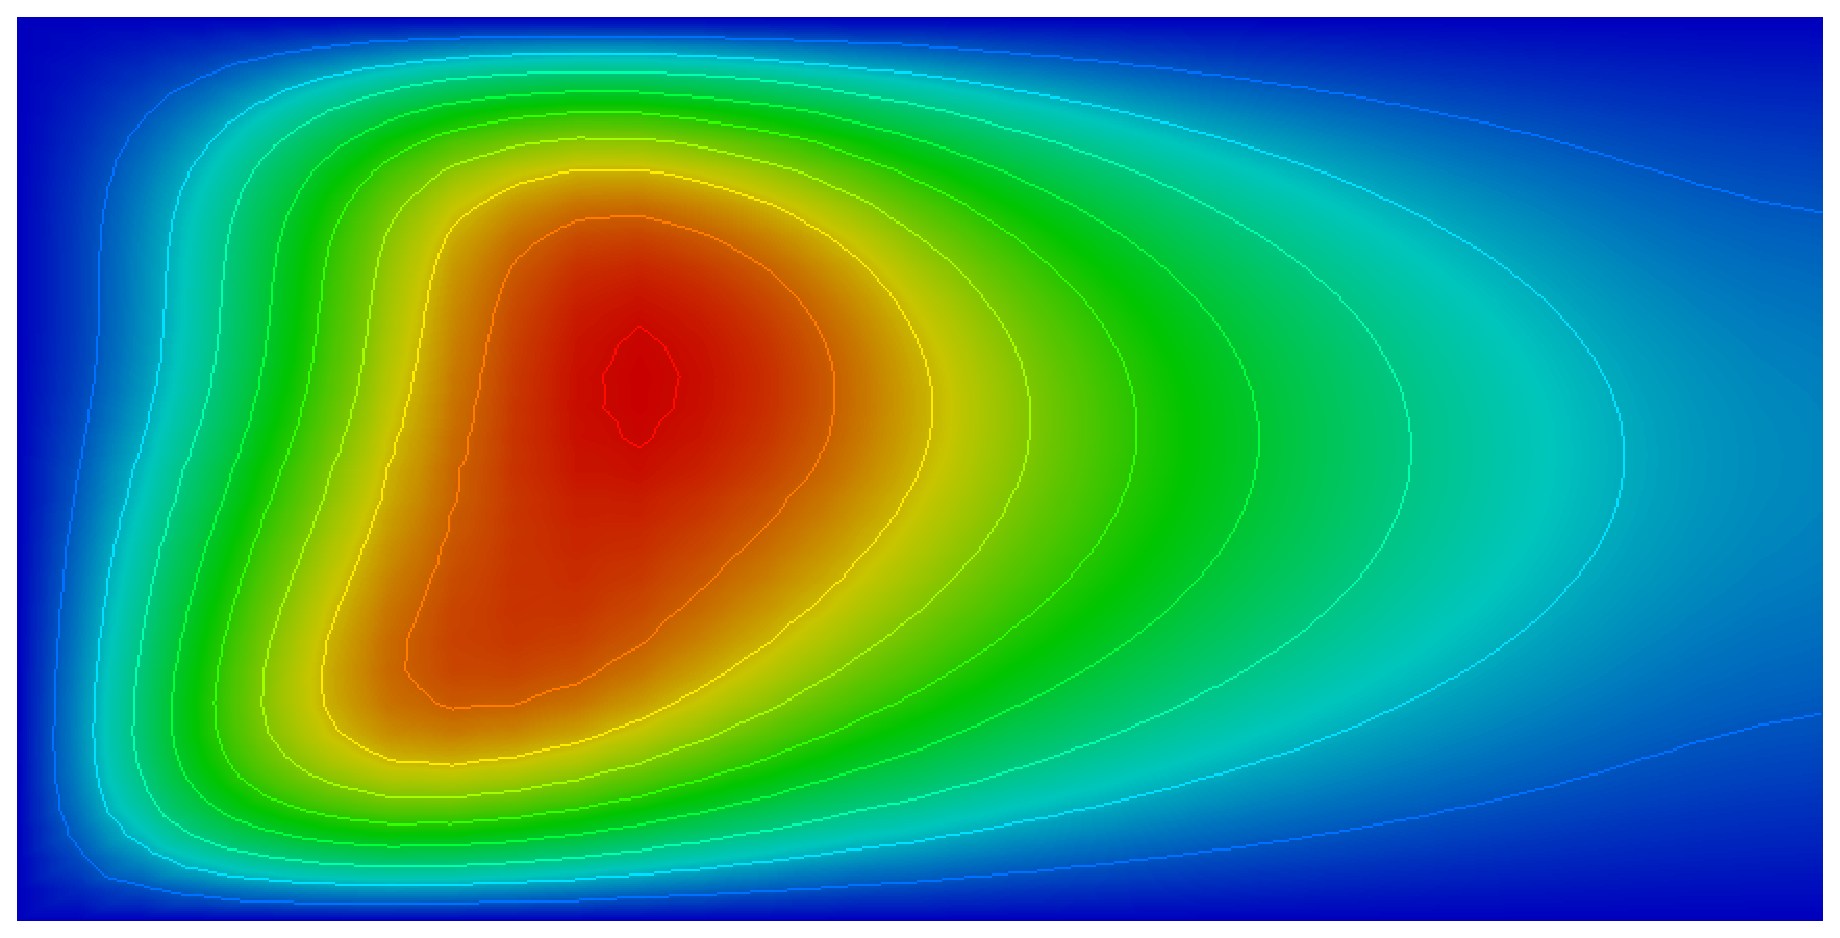
\includegraphics[height=2.8cm,width=5.5cm]{DDDD_ADR/HiMod25slice}}{DDDD_ADR/HiMod25slice}}
\end{figure}
\end{column}

\begin{column}{0.5 \paperwidth}
\begin{figure}
\subfigure[m=16]
{\linkimage{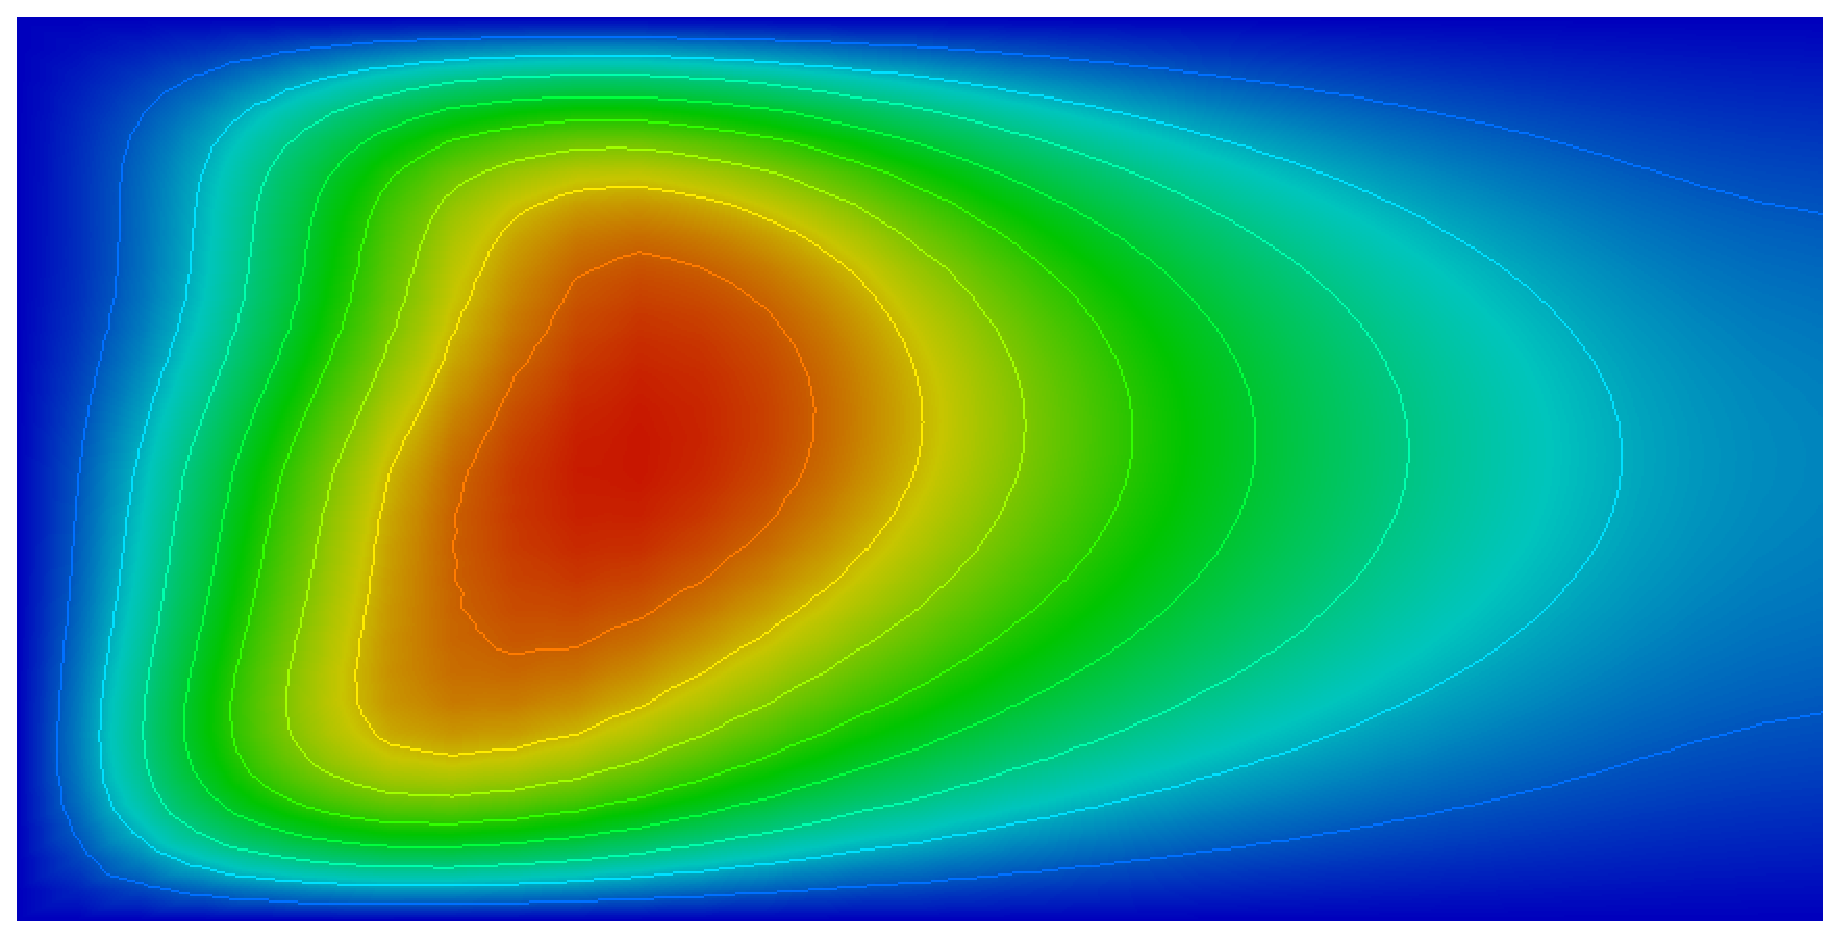
\includegraphics[height=2.8cm,width=5.5cm]{DDDD_ADR/HiMod16slice}}{DDDD_ADR/HiMod16slice}}
\subfigure[FEM]
{\linkimage{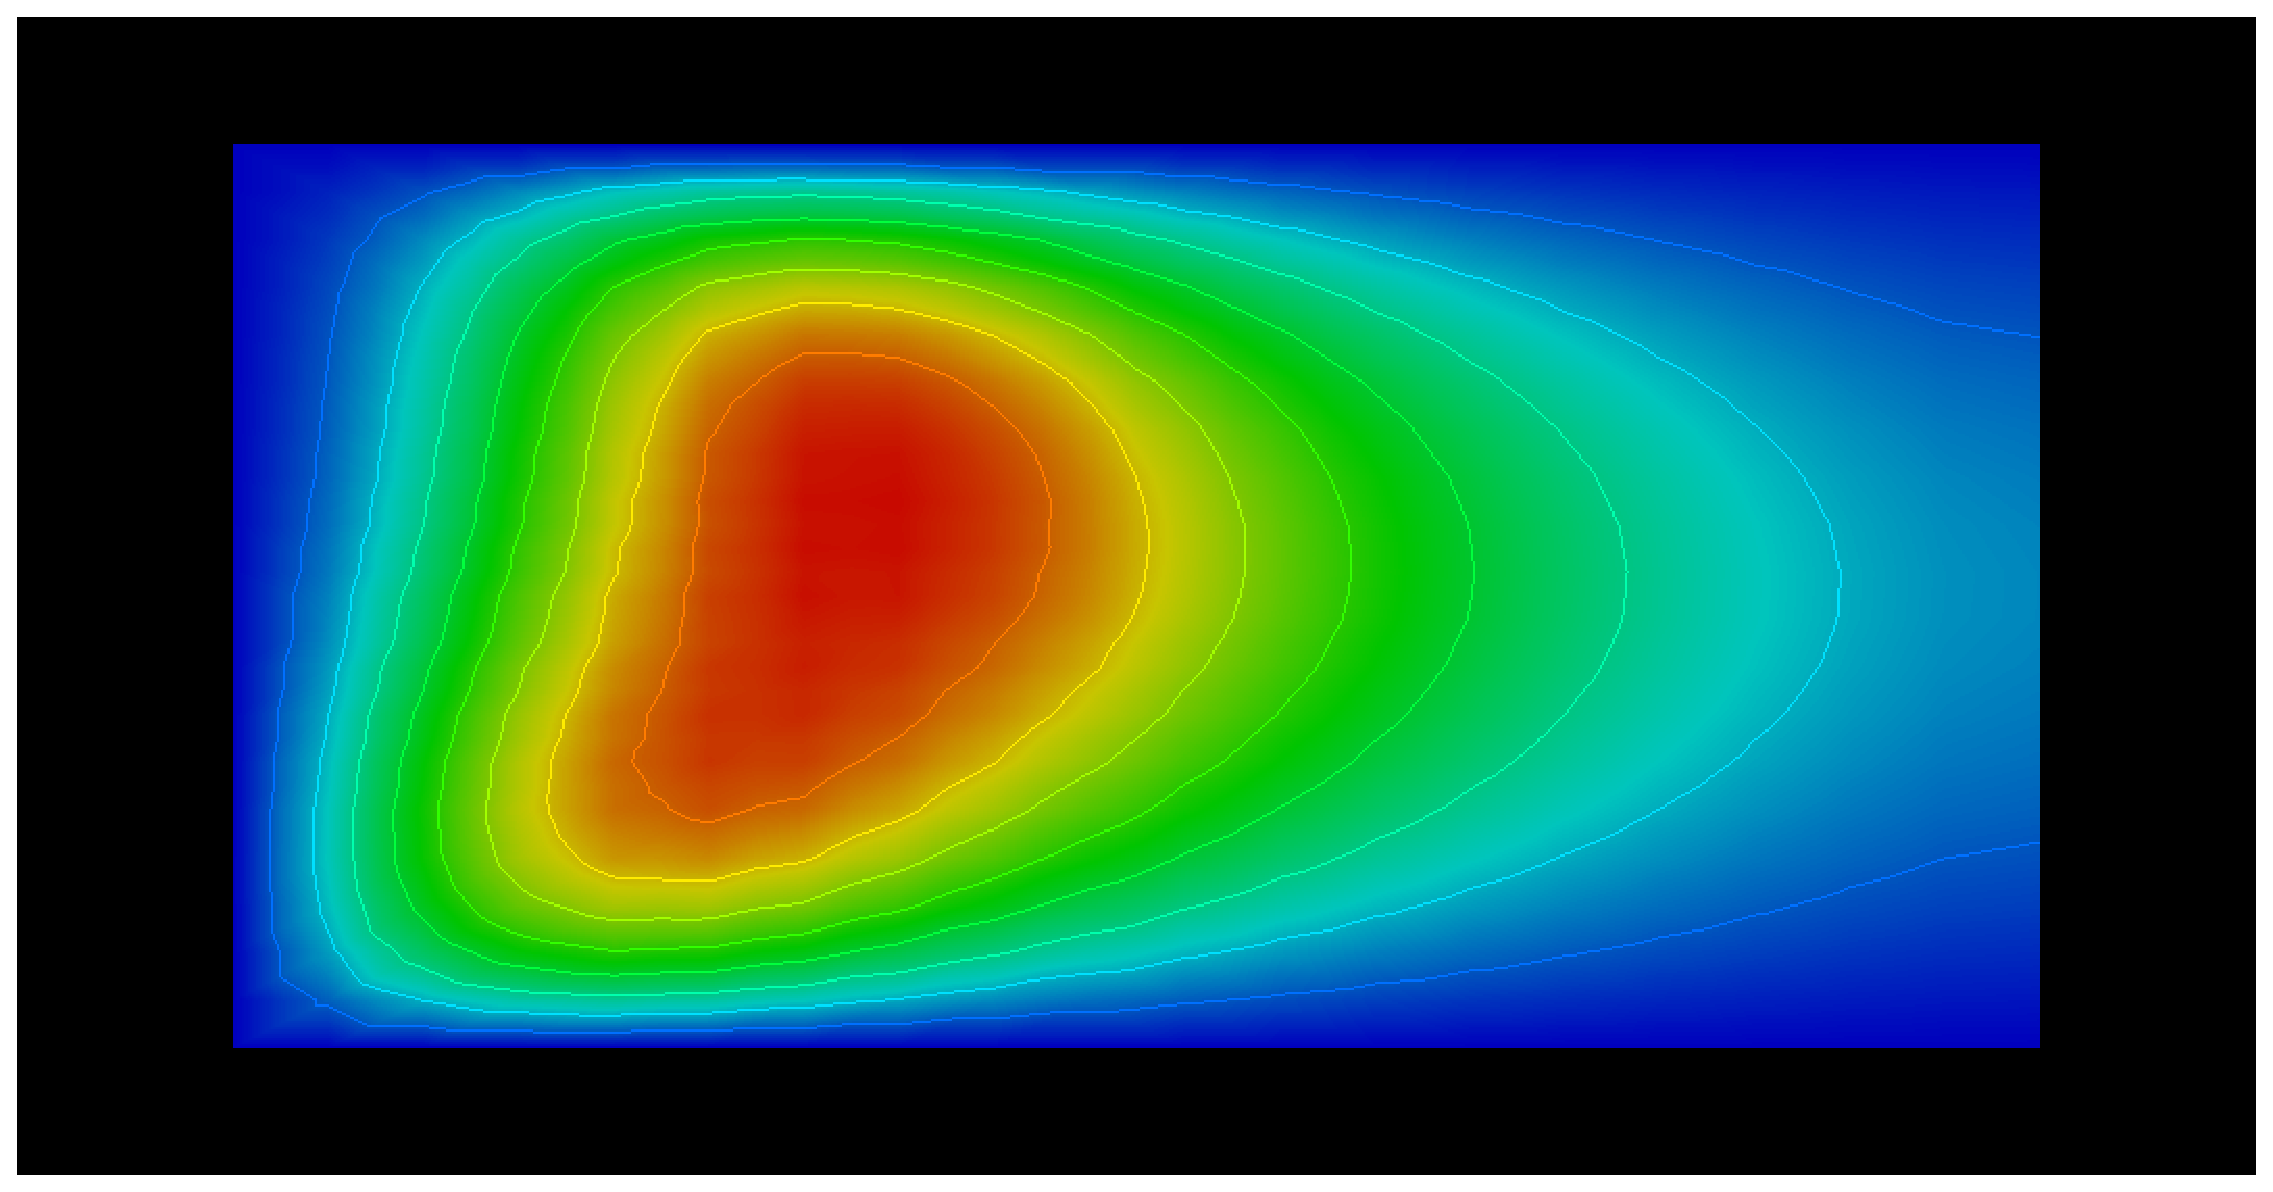
\includegraphics[height=2.8cm,width=5.5cm]{DDDD_ADR/FEMslice}}{DDDD_ADR/FEMslice}}
\end{figure}
\end{column}
\end{columns}


\end{frame}

\begin{frame}
\frametitle{Slice XY}
\begin{columns}

\begin{column}{0.5 \paperwidth}
\begin{figure}
\subfigure[m=9]
{\linkimage{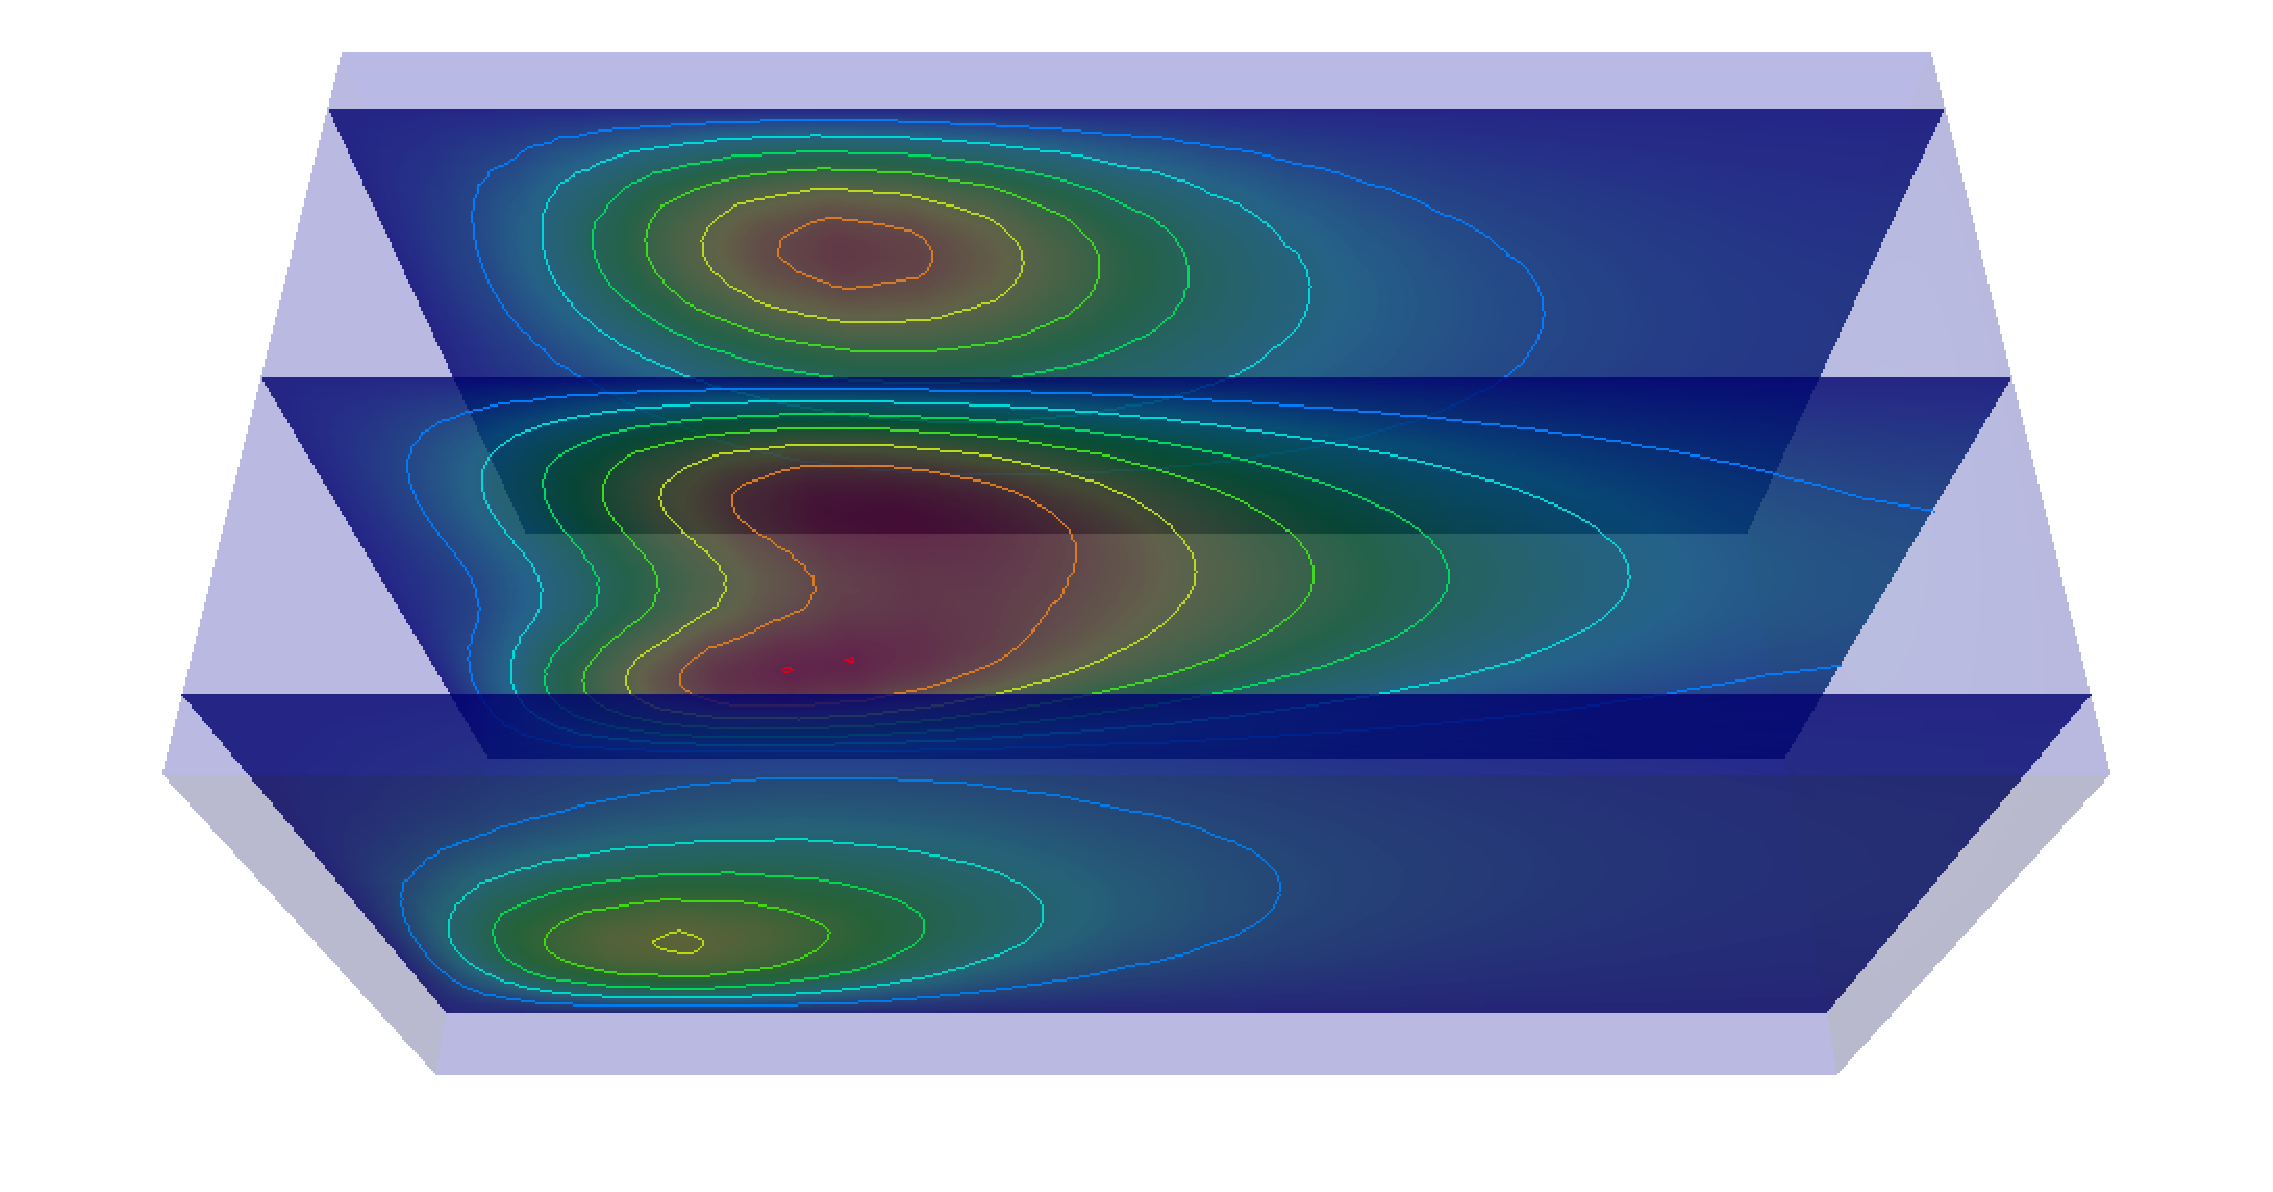
\includegraphics[scale=0.17]{Foto2D+/HiMod_m=9}}{Foto2D+/HiMod_m=9}}
\subfigure[m=25]
{\linkimage{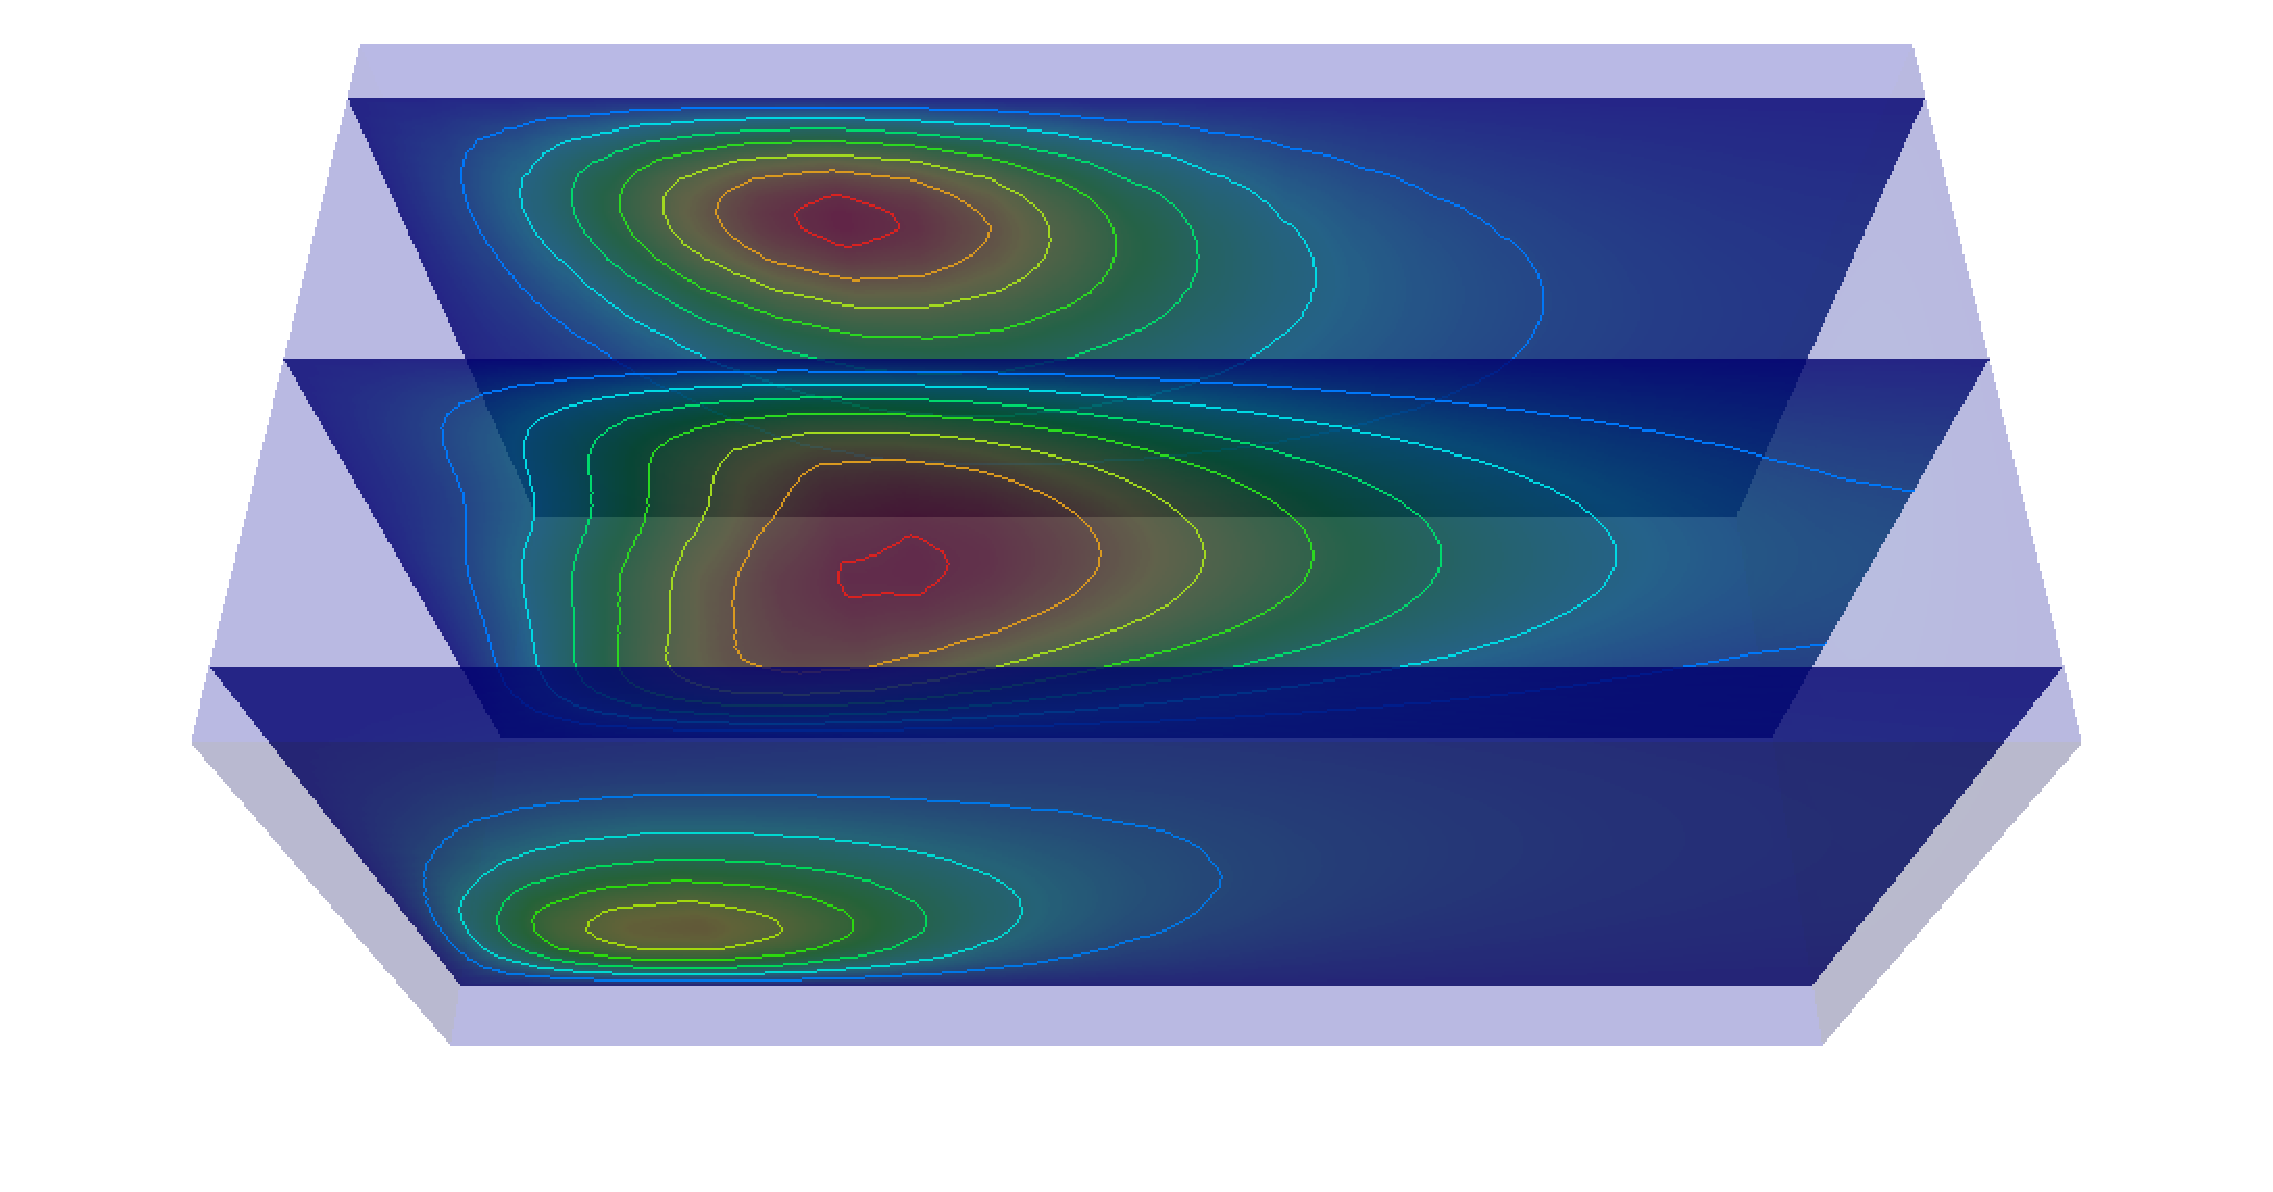
\includegraphics[scale=0.17]{Foto2D+/HiMod_m=16}}{Foto2D+/HiMod_m=16}}
\end{figure}
\end{column}

\begin{column}{0.5 \paperwidth}
\begin{figure}
\subfigure[m=16]
{\linkimage{{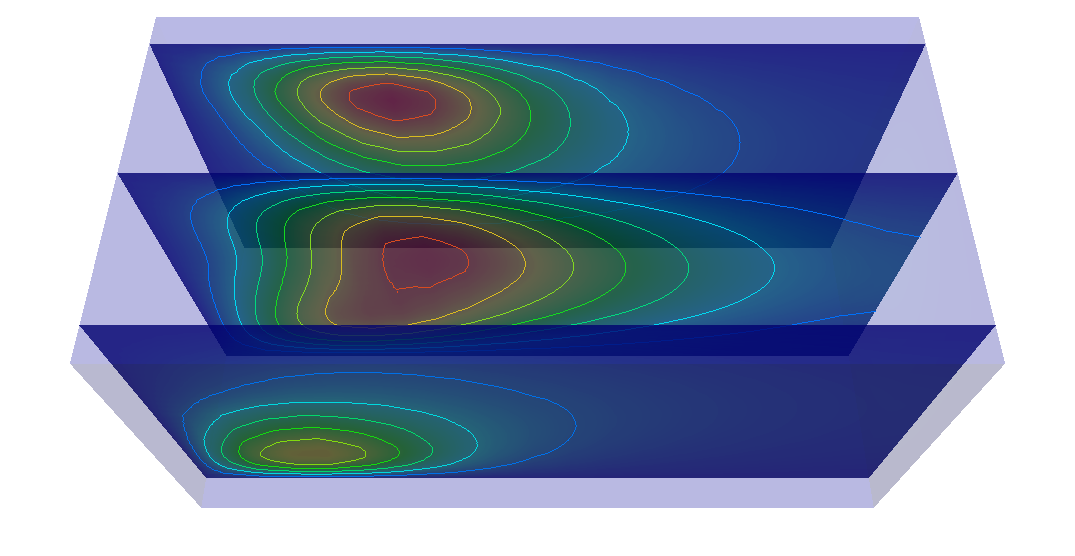
\includegraphics[scale=0.17]{Foto2D+/HiMod_m=25}}}{Foto2D+/HiMod_m=25}}
\subfigure[FEM]
{\linkimage{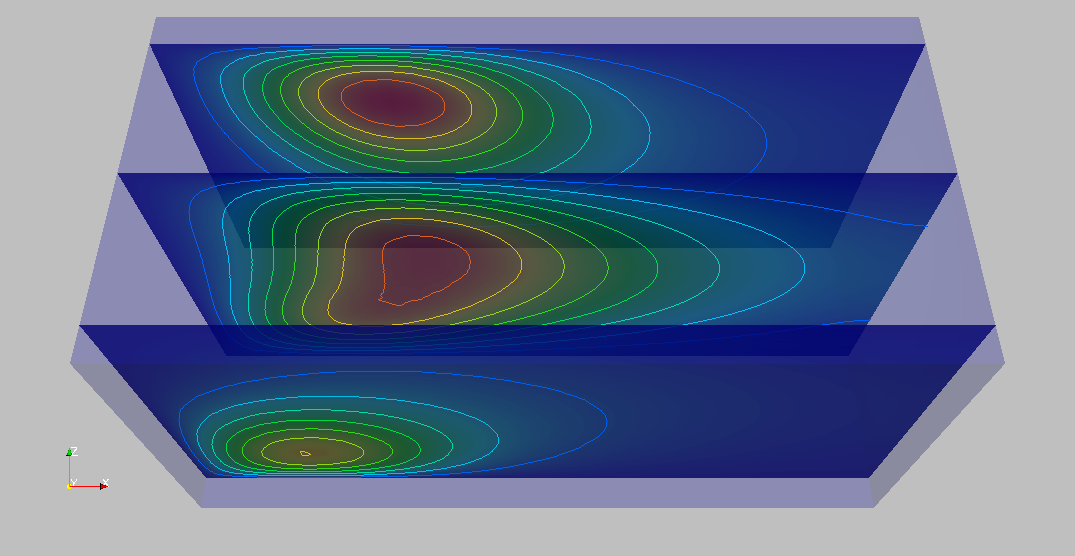
\includegraphics[scale=0.17]{Foto2D+/FEMsolution35}}{Foto2D+/FEMsolution35}}
\end{figure}
\end{column}

\end{columns}
\end{frame}



\subsection{Test di convergenza -- Miste}
